\problemname{Canvas Line}

Your friend Charmion asked you to hang some canvases out to dry on a straight
washing line for an art project she has been working on.
The canvases are artfully arranged such that none of them overlap, although
they may touch along the edges.
For stability, each canvas must be held by two pegs, but because the canvases
are very rigid, they can be held from anywhere.

Each canvas is an integral number of centimetres wide (at least $10$ cm).
Each peg is slightly less than $1$ cm wide. Canvases and pegs are all placed at
integral centimetre positions along the line.

Unnecessary things touching any canvas is a smudge risk, thus every canvas
should be held by exactly two pegs, no more and no less. Given all of the pegs
that are already attached to the line, place as few as possible additional pegs
as necessary to hold all of the canvases.

\begin{figure}[h!]
  \centering
  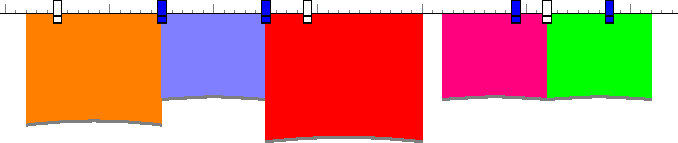
\includegraphics[width=1.0\textwidth]{sample}
  \caption{Illustration of a solution to Sample Input 2. Pre-existing pegs are marked in white.}
  \label{fig:collage}
\end{figure}
\vspace{-0.4cm}

\section*{Input}

The input consists of:
\begin{itemize}
\item One line with an integer $n$ ($1 \leq n \leq 10^3$), the number of
      canvases on the line.
\item $n$ lines, the $i$th of which contains two integers $\ell_i$ and $r_i$
      ($0 \leq \ell_i < r_i \leq 10^9$ and $\ell_i + 10 \le r_i$), the
      positions of the left and the right end of the $i$th canvas in centimetres.
\item One line with an integer $p$ ($0 \leq p \leq 2 \cdot 10^3$), the number of
      pegs already used.
\item One line with $p$ integers $x_1, \ldots, x_p$ ($0 \leq x_i < x_{i+1}
  \leq 10^9$ for each $i$), the position of each existing peg in
    centimetres.
\end{itemize}

Canvases are given from left to right and may touch only at edges,
that is $r_i \le \ell_{i+1}$ for each $i$.

\section*{Output}

If the canvases can be secured, output the smallest number of extra pegs needed
to secure all of the canvases while touching each exactly twice. On the next
line output the integer positions of all of the new pegs.

Otherwise, output ``\texttt{impossible}''.

If there are multiple optimal solutions, you may output any one of them.
